\subsection*{Ejercicio 1}

Un programa para la simulación de sistemas hidráulicos se ejecuta en 122 segundos. Si las operaciones de división con números reales consumen el 73\% de este tiempo, ¿en cuánto se tendría que mejorar la velocidad de estas operaciones si queremos conseguir que dicho programa se ejecute seis veces más rápidamente? ¿Cuál es la ganancia en velocidad máxima que podríamos conseguir si pudiésemos mejorar dichas operaciones tanto como quisiéramos?\\

\begin{itemize}
    \item Sistemas hidráulicos: 122 segundos
    \item Operaciones de división con números reales: 73\% de 122 segundos
    \item Mejora de velocidad: 6 veces
    \item K: Mejora de velocidad de las operaciones de división
\end{itemize}

\begin{equation*}
    S = \frac{T_o}{T_m} = \dfrac{T_o}{(1-0.73)T_o + \dfrac{0.73T_o}{k}}
    = \dfrac{1}{0.27 + \dfrac{0.73}{k}}\leq \dfrac{1}{0.27} = 3,7
\end{equation*}

Por tanto, la ganancia máxima que vamos a poder conseguir mejorando tan solo las operaciones de división con números reales es de 3,7. Si quisiésemos que el programa se ejecutase seis veces más rápidamente, tendríamos que mejorar otros aspectos del sistema.

\textit{Nota:} Estamos aplicando la fórmula de la diapositiva 37-T1:
\begin{equation}
    S = \frac{T_o}{(1-f)T_o + \frac{f x T_o}{K} = \frac{1}{1-f + \frac{f}{K}}}
\end{equation}

\subsection*{Ejercicio 2}

Una mejora en un sitio web ha permitido rebajar de 17 a 9 segundos el tiempo medio de descarga de sus páginas. Si la mejora ha consistido en hacer 3 veces más rápido el subsistema de discos que almacena las páginas del servidor, ¿cuánto tiempo se dedicaba a acceder a los discos antes de realizar la mejora?\\

\begin{itemize}
    \item Rebaja en el tiempo medio de descarga de las páginas: 17 a 9 segundos
    \item Mejora en el subsistema de discos: 3 veces más rápido
    \item Tiempo dedicado a acceder a los discos antes de la mejora: t
    \item $T_o$ = Tiempo medio de descarga antes de la mejora
    \item $T_m$ = Tiempo medio de descarga después de la mejora
    \item f = Fracción de tiempo de descarga de las páginas (que accede al servidor)
\end{itemize}

\begin{equation*}
    T_m = (1-f)T_o + \dfrac{fT_o}{3}\Longrightarrow
    3\cdot \dfrac{T_o-T_m}{2T_o} = f = 3\cdot \dfrac{17-9}{2\cdot 17} = \dfrac{12}{17}
\end{equation*}

Por tanto, antes de la mejora, el tiempo medio de descarga de las páginas que se dedicaba a acceder a los discos era de:
\begin{equation*}
    fT_o = \dfrac{12}{17}\cdot 17 = 12 s
\end{equation*}

\subsection*{Ejercicio 3}

Un computador tarda 100 segundos en ejecutar un programa de simulación de una red de interconexión para multicomputadores. El programa dedica el 20\% en hacer operaciones de aritmética entera (AE), el 30\% en hacer operaciones de aritmética en coma flotante (CF), mientras que el resto se emplea en operaciones de entrada/salida (E/S). Calcule la ganancia en velocidad y el tiempo de ejecución si las operaciones aritméticas enteras y reales se mejoran de manera simultánea 2 y 3 veces, respectivamente.\\

Sea $T_o$ el tiempo de ejecución del programa antes de la mejora, y $T_m$ el tiempo de ejecución del programa después de la mejora. Sea además $f_{AE}$ y $f_{CF}$ las fracciones del tiempo de ejecución del programa que se dedican a las operaciones de aritmética entera y aritmética en coma flotante, respectivamente. Entonces, se tiene:
\begin{align*}
    T_m &= (1-f_{AE}-f_{CF})T_o + \dfrac{f_{AE}T_o}{2} + \dfrac{f_{CF}T_o}{3}
    =\\&= T_o\left[(1-0.2-0.3) + \dfrac{0.2}{2} + \dfrac{0.3}{3}\right]
    = 0.7T_o
    =\\&= 70 s
\end{align*}

Por tanto, la ganancia en velocidad es:
\begin{equation*}
    S = \dfrac{T_o}{T_m} = \dfrac{T_o}{0.7T_o} = \frac{1}{7} \approx 1.43
\end{equation*}

\subsection*{Ejercicio 4}

Una aplicación informática se ejecuta en un computador durante un total de 70 segundos. Mediante el uso de un monitor de actividad se ha podido saber que el 85\% del tiempo se utiliza la tarjeta de red, mientras que el resto del tiempo se hace uso del procesador. Se pide, considerando el sistema original como punto de partida:

\begin{enumerate}
    \item Calcular el incremento de prestaciones si se mejora en 8 veces la velocidad de la tarjeta de red.\\
    
    Sea $T_o$ el tiempo de ejecución del programa antes de la mejora, y $T_m$ el tiempo de ejecución del programa después de la mejora. Sea además $f$ la fracción del tiempo de ejecución del programa que se dedica a la tarjeta de red. Entonces, se tiene:
    \begin{align*}
        T_m &= (1-f)T_o + \dfrac{fT_o}{8}
        =\\&= T_o\left[(1-0.85) + \dfrac{0.85}{8}\right]
        = 0.25625\ T_o
        =\\&= 17.9375s
    \end{align*}

    Por tanto, la ganancia en velocidad es:
    \begin{equation*}
        S = \dfrac{T_o}{T_m} = \dfrac{T_o}{0.25625T_o} = \frac{1}{0.25625} \approx 3.9
    \end{equation*}
    \item Determinar en cuánto hay que mejorar el rendimiento del procesador si se quiere ejecutar la aplicación en 25 segundos.\\
    
    El tiempo que se emplea la tarjeta de red (sin hacer mejoras de esta) es de:
    \begin{equation*}
        fT_o = 0.85\cdot 70 = 59.5s
    \end{equation*}
    Por tanto, mejorando únicamente el rendimiento del procesador, no es posible ejecutar la aplicación en 25 segundos.
\end{enumerate}

\subsection*{Ejercicio 5}

De acuerdo con la ley de Amdahl, deduzca una expresión para la fracción de tiempo $f$ en función de $S$ (el speedup) y $k$ (el número de veces mejorado).\\

La ley de Amdahl establece que la ganancia en velocidad $S$ es:
\begin{multline*}
    S = \dfrac{T_o}{T_m} = \dfrac{T_o}{(1-f)T_o + \dfrac{fT_o}{k}} = \dfrac{1}{1-f + \dfrac{f}{k}}
    \Longrightarrow \dfrac{1}{S}-1=f\left(-1+\dfrac{1}{k}\right)
    \Longrightarrow \\ \Longrightarrow
    f = \dfrac{k(1-S)}{S(1-k)} = \dfrac{k(S-1)}{S(k-1)}\qquad k\neq 1
\end{multline*}

\subsection*{Ejercicio 6}

El administrador de un sistema informático pretende aumentar el rendimiento para evitar que el director del centro lo cese en sus funciones (ha habido más de quince quejas de usuarios en el último mes por el excesivo tiempo de ejecución de los programas). Indíquese, teniendo en cuenta la relación entre prestaciones y coste, qué opción de actualización de un sistema informático, de las dos que se enumeran, resultará más ventajosa:

\begin{enumerate}
    \item Cambio del procesador (250 \euro). Esta modificación permite que el 75\% de los programas se ejecuten dos veces más rápidamente.\\
    
    Sea $T_o$ el tiempo total de ejecución de los programas antes de la actualización, y $T_A$ el tiempo total de ejecución de los programas después de la actualización. Sea además $f$ la fracción de los programas cuya velocidad se vería aumentada (75\% en este caso). Entonces, se tiene:
    \begin{align*}
        T_A &= (1-f)T_o + \dfrac{fT_o}{2}
        =\\&= T_o\left[(1-0.75) + \dfrac{0.75}{2}\right]
        = 0.625\ T_o
    \end{align*}
    \item Ampliación de la memoria principal (150 \euro). La capacidad extra de memoria mejora tres veces el tiempo de ejecución del 40\% de los programas.
    
    Sea $T_o$ el tiempo total de ejecución de los programas antes de la actualización, y $T_B$ el tiempo total de ejecución de los programas después de la actualización. Sea además $f$ la fracción de los programas cuya velocidad se vería aumentada (40\% en este caso). Entonces, se tiene:
    \begin{align*}
        T_B &= (1-f)T_o + \dfrac{fT_o}{3}
        =\\&= T_o\left[(1-0.4) + \dfrac{0.4}{3}\right]
        = \frac{11}{15}\cdot T_o
    \end{align*}
\end{enumerate}

Aunque vemos que la primera alternativa es, de media, un $17.33\%$ más rápida que la segunda, hemos de comparar en función de la relación prestaciones/coste.
\begin{equation*}
    \frac{\nicefrac{\text{Prestaciones}}{\text{Coste}}_A}{\nicefrac{\text{Prestaciones}}{\text{Coste}}_B} = \dfrac{\nicefrac{11}{15}\cdot T_o\cdot 150\text{\euro}}{0.625\cdot T_o\cdot 250\text{\euro}} = \dfrac{88}{125}=0.704
\end{equation*}

Por tanto, la primera alternativa (cambio del procesador) es $0.704$ veces más ventajosa que la segunda. Equivalentemente, y para entendernos, la segunda alternativa es $1.42$ veces (un $42\%$) más ventajosa que la primera. Por tanto, el administrador debería optar por la segunda alternativa, ampliar la memoria principal.

\subsection*{Ejercicio 7}

Un programa de predicción meteorológica tarda 84 minutos en ejecutarse en un supercomputador diseñado al efecto. Sin embargo, esta cantidad de tiempo origina muchos problemas para los estudios de los meteorólogos. El responsable del equipo informático quiere reducir este tiempo sustituyendo la memoria principal por una más rápida, para lo cual existen dos modelos alternativos:

\begin{enumerate}
    \item Modelo Lupita (1100 \euro), que disminuye el tiempo de ejecución hasta los 71 minutos.
    \item Modelo Lucho (1300 \euro), que rebaja este tiempo de ejecución hasta los 63 minutos.
\end{enumerate}
Determine cuál de los dos modelos anteriores representa la mejor opción ateniéndonos a la relación prestaciones/coste. Exprese el resultado como ``\% de mejora en la relación prestaciones/coste''.\\

La comparación de la relación prestaciones/coste de los dos modelos es:
\begin{equation*}
    \frac{\nicefrac{\text{Prestaciones}}{\text{Coste}}_{\text{Lupita}}}{\nicefrac{\text{Prestaciones}}{\text{Coste}}_{\text{Lucho}}} = \dfrac{63\cdot 1300}{71\cdot 1100} = \dfrac{819}{781} \approx 1.049
\end{equation*}

Por tanto, el modelo Lupita es $1.049$ veces (un $4.9\%$) más ventajoso que el modelo Lucho.

\subsection*{Ejercicio 8}

El tiempo medio de respuesta de un sitio web es de 15 segundos. Mediante un monitor software se ha podido determinar que el 55\% de este tiempo es utilizado por el subsistema de discos, mientras que el resto se dedica a la ejecución de los scripts en el procesador de 2 GHz de que dispone el servidor. El administrador del sitio, después de soportar estoicamente las quejas de los usuarios, pretende reducir este tiempo por debajo de los 11 segundos. ¿Cuál de las dos opciones planteadas a continuación consigue este objetivo?

\begin{enumerate}
    \item Adquirir un nuevo procesador que trabaja a 3 GHz.
    
    Sea $T_o$ el tiempo de respuesta del sitio web antes de la actualización, y $T_A$ el tiempo de respuesta del sitio web después de la actualización. Sea además $f$ la fracción del tiempo de respuesta del sitio web que se dedica a la ejecución de los scripts en el procesador. Entonces, se tiene:
    \begin{align*}
        T_A &= (1-f)T_o + fT_o\cdot \dfrac{2}{3}
        =\\&= T_o\left[(1-0.45) + 0.45\cdot \dfrac{2}{3}\right]
        = 0.85\ T_o
        =\\&= 12.75s
    \end{align*}
    \item Substituir el subsistema de discos por uno de segunda mano $2.5$ veces más rápido que el actual.
    
    Sea $T_o$ el tiempo de respuesta del sitio web antes de la actualización, y $T_B$ el tiempo de respuesta del sitio web después de la actualización. Sea además $f$ la fracción del tiempo de respuesta del sitio web que se dedica al subsistema de discos. Entonces, se tiene:
    \begin{align*}
        T_B &= (1-f)T_o + fT_o\cdot \dfrac{1}{2.5}
        =\\&= T_o\left[(1-0.55) + 0.55\cdot \dfrac{1}{2.5}\right]
        = 0.67\ T_o
        =\\&= 10.05s
    \end{align*}
\end{enumerate}

Por tanto, la segunda opción es la que consigue el objetivo de reducir el tiempo de respuesta por debajo de los 11 segundos.

\subsection*{Ejercicio 9}
Un programa de simulación de sistemas aerodinámicos de control se ejecuta en 280 segundos. El 70\% del tiempo de ejecución se utiliza el procesador; el resto se dedica a acceder al subsistema de discos. Un incremento del presupuesto aportado por el ministerio ha permitido adquirir un nuevo procesador tres veces más rápido.

\begin{enumerate}
    \item Determine el tiempo de ejecución del simulador después de actualizar el procesador.
    
    Sea $T_o$ el tiempo de ejecución del programa antes de la actualización, y $T_m$ el tiempo de ejecución del programa después de la actualización. Sea además $f$ la fracción del tiempo de ejecución del programa que se dedica al procesador. Entonces, se tiene:
    \begin{align*}
        T_m &= (1-f)T_o + fT_o\cdot \dfrac{1}{3}
        =\\&= T_o\left[(1-0.7) + 0.7\cdot \dfrac{1}{3}\right]
        = \dfrac{8}{15}\ T_o
        =\\&= 149.33s
    \end{align*}
    \item Calcule ahora, esto es, después de haber hecho la actualización del procesador, cuál es la fracción del tiempo mejorado de ejecución durante el cual se utiliza el nuevo procesador. Haga un análisis del fenómeno observado.
    
    La fracción del tiempo de ejecución mejorado de ejecución durante el cual se utiliza el nuevo procesador es:
    \begin{equation*}
        f_m = 1-\dfrac{(1-0.7)T_o}{T_m} = 1-\dfrac{0.3T_o}{\nicefrac{8}{15}T_o} = 0.4375
    \end{equation*}

    El tiempo dedicado a acceder al subsistema de discos se mantiene constante, pero el tiempo dedicado a la ejecución de los scripts en el procesador se reduce del 70\% al 43.75\%. Por tanto, anteriormente sí era vital mejorar dicho componente, pero ahora, con el nuevo procesador, es más importante mejorar el subsistema de discos.
    \item A raíz del resultado obtenido en el apartado anterior, si hubiéramos de mejorar este sistema actualizado, ¿sobre qué componente del mismo deberíamos incidir? Justifique numéricamente la respuesta.
    
    Como hemos indicado, y debido a que siempre hemos de priorizar mejorar el componente que más tiempo de ejecución consume, deberíamos incidir sobre el subsistema de discos.
\end{enumerate}

\subsection*{Ejercicio 10}
Un equipo de biólogos que investiga sobre clonación de células utiliza el multiprocesador ALLIANT para ejecutar un simulador que se puede paralelizar en una fracción $f$ de su tiempo de ejecución. La Figura~\ref{fig:1_10} presenta la ganancia en velocidad conseguida por la máquina paralela en la ejecución del simulador para diferentes valores del número de procesadores ($p$).\\

\begin{figure}
    \centering
    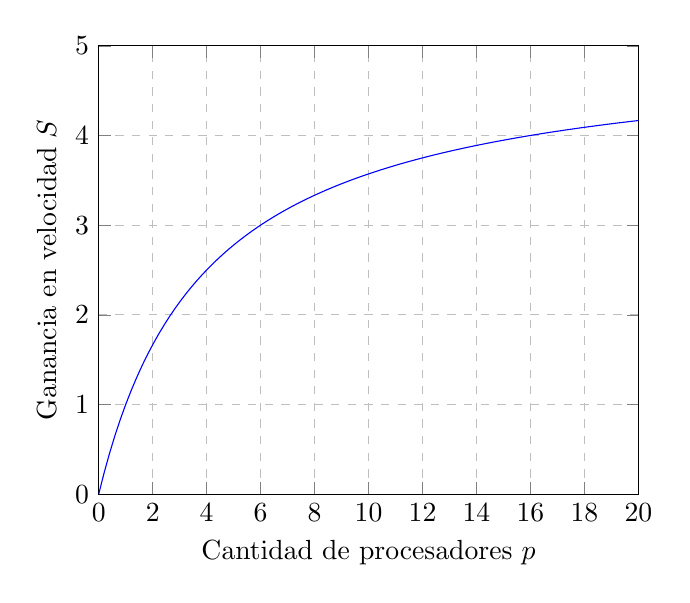
\begin{tikzpicture}
        \begin{axis}[
            xlabel={Cantidad de procesadores $p$},
            ylabel={Ganancia en velocidad $S$},
            xmin=0, xmax=20,
            ymin=0, ymax=5,
            xtick={0,2,4,6,8,10,12,14,16,18,20},
            ytick={0,1,2,3,4,5},
            ymajorgrids=true,
            xmajorgrids=true,
            grid style=dashed,
        ]

        % Gráfica de y=1/(1-x+x/4)
        \addplot[domain=0:20, samples=100, color=blue]{1/(1-0.8+0.8/x)};
            
        \end{axis}
    \end{tikzpicture}
    \caption{Ganancia en velocidad ($S$) en función del número de procesadores ($p$).}
\end{figure}

\begin{enumerate}
    \item ¿Cuál es la fracción paralelizable $f$ del programa de simulación?
    
    El tiempo mejorado, $T_m$, es:
    \begin{equation*}
        T_m = (1-f)T_o + \dfrac{fT_o}{p}
    \end{equation*}

    Por tanto, la ganancia en velocidad $S$ en función del número de procesadores $p$ es:
    \begin{equation*}
        S = \dfrac{T_o}{T_m} = \dfrac{T_o}{(1-f)T_o + \dfrac{fT_o}{p}} = \dfrac{1}{1-f + \dfrac{f}{p}}
    \end{equation*}

    Despejando $f$ de forma análoga al ejercicio 5 se obtiene:
    \begin{equation*}
        f = \dfrac{p(S-1)}{S(p-1)}
    \end{equation*}

    Empleando tanto los puntos $(6,3)$ como $(16,4)$, se obtiene en ambos casos:
    \begin{equation*}
        f = \dfrac{4}{5} = 0.8
    \end{equation*}
    \item Si la parte secuencial (es decir, la no paralelizable) del simulador se ejecuta en 65s, ¿cuánto tiempo han de esperar los biólogos para obtener los resultados de la simulación con una configuración de 6 procesadores?
    
    Como el $20\%$ del tiempo total de ejecución (en el caso de un único procesador) se dedica a la parte secuencial, el tiempo de ejecución del simulador en dicho únco procesador es:
    \begin{equation*}
        0.2T_o = 65s\Longrightarrow T_o = 325s
    \end{equation*}

    Por tanto, el tiempo de ejecución del simulador en un sistema con 6 procesadores es:
    \begin{equation*}
        T_m = (1-f)T_o + \dfrac{fT_o}{6} = 0.2T_o + \dfrac{0.8T_o}{6} = T_o\left(0.2 + \dfrac{0.8}{6}\right) = \dfrac{T_o}{3} = 108.33s
    \end{equation*}
    \item Los científicos pretenden obtener resultados del simulador en un tiempo máximo de 70s sin modificar el código del programa. Si el sistema ALLIANT está preparado para ampliar el número de procesadores hasta $p = 30$, ¿podrán conseguir los biólogos su objetivo?
    
    El tiempo de ejecución del simulador en un sistema con 30 procesadores sería:
    \begin{equation*}
        T_m = (1-f)T_o + \dfrac{fT_o}{30} = 0.2T_o + \dfrac{0.8T_o}{30} = T_o\left(0.2 + \dfrac{0.8}{30}\right) = \dfrac{17}{75}T_o = 73.67s
    \end{equation*}

    Por tanto, los biólogos no podrán conseguir su objetivo, puesto que el tiempo de ejecución del simulador en un sistema con 30 procesadores es mayor que su objetivo.\\

    Veamos cuántos procesadores necesitarían para conseguir su objetivo:
    \begin{equation*}
        T_m = (1-f)T_o + \dfrac{fT_o}{p} = 0.2T_o + \dfrac{0.8T_o}{p}\leq 70\iff
        65+\dfrac{260}{p}\leq 70\iff p\geq \dfrac{260}{5} = 52
    \end{equation*}

    Por tanto, necesitarían al menos 52 procesadores para conseguir su objetivo.
    \item Un informático afirma que el sistema ALLIANT podría conseguir el objetivo anterior con $p = 6$ procesadores si se reduce a la mitad la fracción secuencial (es decir, no paralelizable) del simulador. ¿Es válida esta propuesta?
    
    Supongamos ahora que el tiempo secuencial es tan solo el $10\%$ del tiempo total de ejecución con un único procesador; es decir, $f = 0.9$. En este caso, el tiempo de ejecución del simulador en un sistema con 6 procesadores sería:
    \begin{equation*}
        T_m = (1-f)T_o + \dfrac{fT_o}{6} = 0.1T_o + \dfrac{0.9T_o}{6} = T_o\left(0.1 + \dfrac{0.9}{6}\right) = \dfrac{T_o}{4} = 81.25s
    \end{equation*}

    Por tanto, la propuesta no es válida, ya que el tiempo de ejecución del simulador en un sistema con 6 procesadores sería mayor que su objetivo.
\end{enumerate}

\subsection*{Ejercicio 11}
Ante la necesidad de reducir el tiempo de ejecución de un programa de cálculo de trayectorias espaciales, un equipo de arquitectos de computadores ha diseñado un nuevo procesador que mejora 3 veces la ejecución de las operaciones de coma flotante. El programa, cuando se ejecuta utilizando este nuevo procesador, emplea el 65\% del tiempo en la realización de operaciones de coma flotante.

\begin{enumerate}
    \item Calcule qué tanto por ciento del tiempo de ejecución necesitaban las operaciones de coma flotante en el sistema con el procesador original.
    
    Sea $f$ la fracción del tiempo de ejecución del programa original que se dedica a las operaciones de coma flotante. Entonces, se tiene:
    \begin{align*}
        T_m &= (1-f)T_o + \dfrac{fT_o}{3}\\
        0.65T_m &= \dfrac{fT_o}{3}
    \end{align*}

    Por tanto, tenemos que $fT_o=1.95T_m$. Por tanto:
    \begin{equation*}
        T_m = T_o - 1.95T_m + 0.65T_m\Longrightarrow
        2.3T_m = T_o
    \end{equation*}

    Por tanto, tenemos que:
    \begin{equation*}
        0.65\cdot \dfrac{T_o}{2.3} = \dfrac{fT_o}{3}\Longrightarrow
        f = 3\cdot \dfrac{0.65}{2.3} = \dfrac{39}{46}\approx 0.848
    \end{equation*}

    Por tanto, el $84.8\%$ del tiempo de ejecución necesitaban las operaciones de coma flotante en el sistema con el procesador original.
    \item Indique cuál es la ganancia en velocidad global conseguida por el nuevo procesador.
    
    Tenemos que:
    \begin{equation*}
        S = \dfrac{T_o}{T_m} = \dfrac{2.3T_m}{T_m} = 2.3
    \end{equation*}
\end{enumerate}

\subsection*{Ejercicio 12}

La gráfica de la Figura~\ref{fig:1_2} muestra la ganancia en velocidad (speedup), calculada mediante la ley de Amdahl, que se consigue en un computador después de reemplazar la vieja unidad de disco por una nueva, en función de la fracción del tiempo de ejecución en el que se usaba la antigua unidad.

\begin{figure}[H]
    \centering
    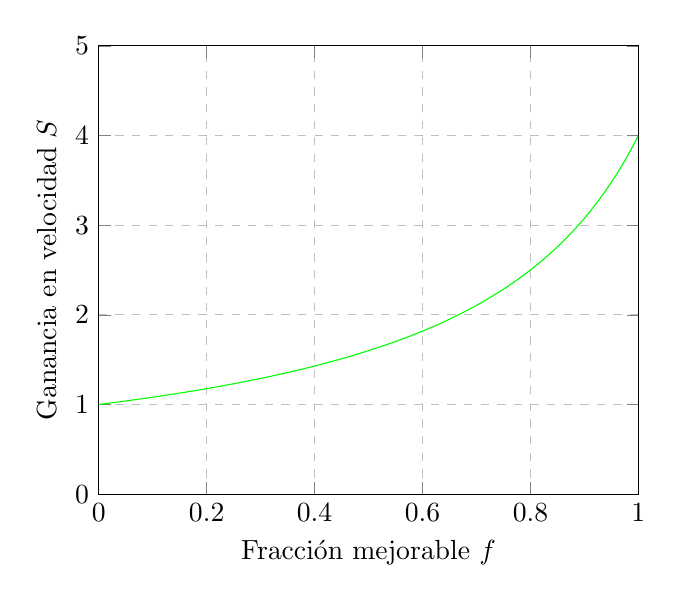
\begin{tikzpicture}
        \begin{axis}[
            xlabel={Fracción mejorable $f$},
            ylabel={Ganancia en velocidad $S$},
            xmin=0, xmax=1,
            ymin=0, ymax=5,
            xtick={0,0.2,0.4,0.6,0.8,1},
            ytick={0,1,2,3,4,5},
            ymajorgrids=true,
            xmajorgrids=true,
            grid style=dashed,
        ]

        % Gráfica de y=1/(1-x+x/4)
        \addplot[domain=0:1, samples=100, color=green]{1/(1-x+x/4)};
            
        \end{axis}
    \end{tikzpicture}
    \caption{Ganancia en velocidad ($S$) en función de la fracción mejorable ($f$).}
    \label{fig:1_2}
\end{figure}

\begin{enumerate}
    \item Indique cuántas veces es más rápida la nueva unidad de disco respecto de la que se ha retirado del computador.
    
    Tenemos que:
    \begin{equation*}
        S = \dfrac{1}{1-f+\dfrac{f}{k}}
    \end{equation*}

    Empleando el punto $(1,4)$, se tiene:
    \begin{equation*}
        4 = \dfrac{1}{1-1+\dfrac{1}{k}}\Longrightarrow k = 4
    \end{equation*}

    Por tanto, la nueva unidad de disco es 4 veces más rápida que la vieja.
    \item El computador, antes de hacer la actualización, tardaba 126 segundos en ejecutar la aplicación. Determine, en el mejor de los casos, cuál sería el tiempo de ejecución en el sistema actualizado. Justifique la respuesta.
    
    Tenemos que:
    \begin{equation*}
        T_m = (1-f)T_o + \dfrac{fT_o}{4} = T_o\left(1-f+\dfrac{f}{4}\right)
    \end{equation*}

    El mejor de los casos sería suponer que la fracción del tiempo de ejecución en el que se usaba la antigua unidad era la máxima posible, es decir, $f=1$. Por tanto, el tiempo de ejecución en el sistema actualizado sería:
    \begin{equation*}
        T_m = \dfrac{T_o}{4} = 31.5s
    \end{equation*}
    \item Dibuje sobre la misma gráfica la curva que se obtendría si la nueva unidad de disco fuera 2 veces más rápida que la vieja.
    
    La gráfica obtenida se encuentra en la Figura~\ref{fig:1_2_solucion}, y vendría dada por la ecuación:
    \begin{equation*}
        S = \dfrac{1}{1-f+\dfrac{f}{2}}
    \end{equation*}

    \begin{figure}
        \centering
        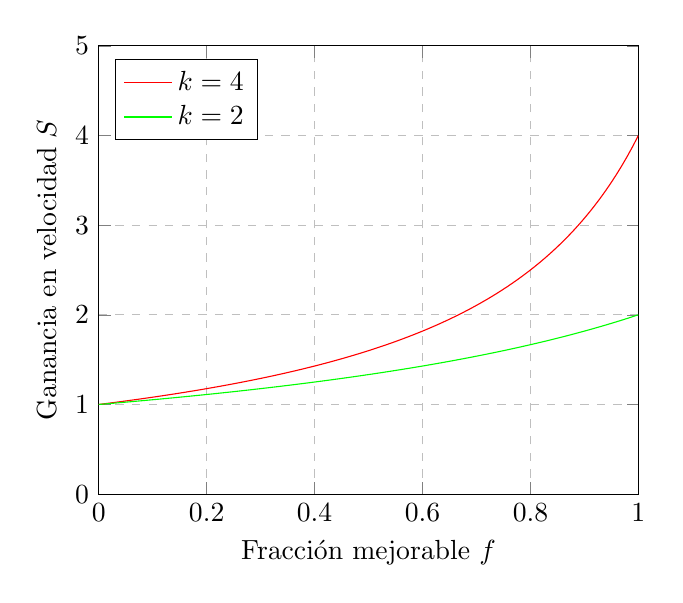
\begin{tikzpicture}
            \begin{axis}[
                xlabel={Fracción mejorable $f$},
                ylabel={Ganancia en velocidad $S$},
                xmin=0, xmax=1,
                ymin=0, ymax=5,
                xtick={0,0.2,0.4,0.6,0.8,1},
                ytick={0,1,2,3,4,5},
                ymajorgrids=true,
                xmajorgrids=true,
                grid style=dashed,
                legend pos=north west
            ]

            \addplot[domain=0:1, samples=100, color=red]{1/(1-x+x/4)};
            \addlegendentry{$k=4$}
    
            % Gráfica de y=1/(1-x+x/2)
            \addplot[domain=0:1, samples=100, color=green]{1/(1-x+x/2)};
            \addlegendentry{$k=2$}
                
            \end{axis}
        \end{tikzpicture}
        \caption{Ganancia en velocidad ($S$) en función de la fracción mejorable ($f$).}
        \label{fig:1_2_solucion}
    \end{figure}

\end{enumerate}

\subsection*{Ejercicio 13}
Una aplicación informática se ejecuta en un computador durante un total de 70s. Mediante el uso de un monitor de actividad se ha podido saber que durante el 85\% del tiempo de ejecución se utiliza la CPU (CPUo), mientras que el resto del tiempo se hace uso del disco duro (DD). Determine cuántas veces debe ser, como mínimo, más rápido un procesador (CPUm) que cuesta el doble que el procesador actual para que hubiese valido la pena comprarlo en lugar de éste ateniéndonos a la relación prestaciones del sistema/coste del procesador.\\

Sea $k$ el número de veces más rápido que el procesador actual ha de ser el nuevo procesador. Entonces, se tiene:
\begin{align*}
    T_m &= (1-f)T_o + \dfrac{fT_o}{k}
    =\\&= T_o\left[(1-0.85) + 0.85\cdot \dfrac{1}{k}\right]
    = T_o\left[0.15 + \dfrac{0.85}{k}\right]
\end{align*}

Tenemos por tanto que:
\begin{align*}
    \dfrac{\nicefrac{\text{Prestaciones}}{\text{Coste}}_{\text{CPUm}}}{\nicefrac{\text{Prestaciones}}{\text{Coste}}_{\text{CPUo}}} &= \dfrac{T_o}{T_m}\cdot \dfrac{\text{Coste}_{\text{CPUo}}}{\text{Coste}_{\text{CPUm}}}
    = \dfrac{1}{0.15 + \dfrac{0.85}{k}}\cdot \dfrac{1}{2}  \geq 1\iff 
    \\ &\iff 1-0.3\geq \dfrac{1.7}{k}\iff k\geq \dfrac{1.7}{0.7} \approx 2.4286
\end{align*}

Por tanto, el nuevo procesador ha de ser al menos 2.43 veces más rápido que el procesador actual para que hubiese valido la pena comprarlo en lugar de éste.

\subsection*{Ejercicio 14}

Se sabe que el tiempo de respuesta de una petición a un servidor de bases de datos es de 23 segundos, y que el 72\% de ese tiempo se emplea en acceder al subsistema de discos, cuyo coste es de 3500 \euro. Con el objetivo de mejorar las prestaciones del servidor, un ingeniero en informática está estudiando la posibilidad de adquirir, en su lugar, otro subsistema de discos tres veces más rápido pero con un coste de 4800 \euro.

\begin{enumerate}
    \item Calcúlese el nuevo tiempo de respuesta del servidor con el subsistema de discos más caro.
    
    El tiempo de respuesta del servidor con el subsistema de discos más caro sería:
    \begin{align*}
        T_m &= (1-f)T_o + \dfrac{fT_o}{3} = T_o\left(1-f+\dfrac{f}{3}\right)
        =\\&= \dfrac{13}{25}\ T_o = 11.96s
    \end{align*}
    \item ¿Merece la pena comprar el sub-sistema de discos más caro ateniéndonos exclusivamente a la relación prestaciones/coste?
    
    Tenemos que:
    \begin{equation*}
        \dfrac{\nicefrac{\text{Prestaciones}}{\text{Coste}}_{\text{caro}}}{\nicefrac{\text{Prestaciones}}{\text{Coste}}_{\text{barato}}} = \dfrac{T_o}{T_m}\cdot \dfrac{\text{Coste}_{\text{barato}}}{\text{Coste}_{\text{caro}}}
        = \dfrac{T_o}{\nicefrac{13}{25}\ T_o}\cdot \dfrac{3500}{4800} \approx 1.4022
    \end{equation*}

    Por tanto, sí merece la pena comprar el sub-sistema de discos más caro.
    \item ¿Cuál es la mejora máxima teórica que se podría alcanzar en el tiempo de respuesta manteniendo el subsistema de discos más barato y mejorando el resto de componentes? Exprese el resultado en “número de segundos más rápido” y en “número de veces más rápido”.
    
    Suponiendo ahora que $f=1-0.72=0.28$ y que $k$ es la mejora, se tiene:
    \begin{equation*}
        T_m = (1-f)T_o + \dfrac{fT_o}{k} = 0.72T_o + \dfrac{0.28T_o}{k}\geq 0.72T_o=16.56s
    \end{equation*}

    Por tanto, tenemos que:
    \begin{equation*}
        T_o-T_m \leq 23-16.56 = 6.44s
    \end{equation*}
    Es decir, la mejora máxima teórica haría que el tiempo de respuesta fuese $6.44s$ más rápido que el original. Por otro lado, se tiene:
    \begin{equation*}
        \dfrac{T_o}{T_m}\leq \dfrac{T_o}{0.72T_o} = \dfrac{25}{18} \approx 1.39
    \end{equation*}
    Por tanto, la mejora máxima teórica haría que el tiempo de respuesta fuese $1.39$ veces más rápido que el original.
\end{enumerate}

\subsection*{Ejercicio 15}

Un computador tarda 1000 segundos en ejecutar un proceso de formateo y conversión de imágenes. De todo ese tiempo, el programa dedica un 30\% en hacer operaciones de aritmética en coma flotante, y 250s en accesos al subsistema de discos.

\begin{enumerate}
    \item Calcule la ganancia en velocidad que se consigue si añadimos al equipo una GPU de 500\euro~capaz de ejecutar las operaciones en coma flotante 10 veces más rápido.
    
    Tenemos que:
    \begin{align*}
        T_m &= (1-f)T_o + \dfrac{fT_o}{10} = T_o\left(1-f+\dfrac{f}{10}\right)
        =\\&= 0.73\ T_o
    \end{align*}

    Por tanto, la ganancia en velocidad que se consigue es de:
    \begin{equation*}
        S = \dfrac{T_o}{T_m} = \dfrac{T_o}{0.73\ T_o} = \dfrac{100}{73} \approx 1.37
    \end{equation*}
    \item Calcule la ganancia en velocidad que se consigue con respecto al tiempo original si remplazamos el subsistema de discos por otro cuyo precio es de 400\euro~y consigue que los accesos al mismo sean 5 veces más rápidos.
    
    La francción del tiempo original que se dedica al subsistema de discos es:
    \begin{equation*}
        f = \dfrac{250}{1000} = 0.25
    \end{equation*}

    Por tanto, el tiempo de ejecución del proceso con el nuevo subsistema de discos sería:
    \begin{align*}
        T_m &= (1-f)T_o + \dfrac{fT_o}{5} = T_o\left(1-f+\dfrac{f}{5}\right)
        =\\&= 0.8\ T_o
    \end{align*}

    Por tanto, la ganancia en velocidad que se consigue es de:
    \begin{equation*}
        S = \dfrac{T_o}{T_m} = \dfrac{T_o}{0.8\ T_o} = \dfrac{5}{4} = 1.25
    \end{equation*}
    \item Calcule la ganancia en velocidad que se consigue utilizando simultáneamente las dos mejoras de los apartados anteriores.
    
    El tiempo de ejecución del proceso con las dos mejoras sería:
    \begin{align*}
        T_m &= (1-f_{\text{CPU}}-f_{\text{DD}})T_o + \dfrac{f_{\text{CPU}}T_o}{10} + \dfrac{f_{\text{DD}}T_o}{5}
        =\\&= T_o\left(1-f_{\text{CPU}}-f_{\text{DD}}+\dfrac{f_{\text{CPU}}}{10}+\dfrac{f_{\text{DD}}}{5}\right)
        =\\&= 0.53\ T_o
    \end{align*}

    Por tanto, la ganancia en velocidad que se consigue es de:
    \begin{equation*}
        S = \dfrac{T_o}{T_m} = \dfrac{T_o}{0.53\ T_o} = \dfrac{100}{53} \approx 1.89
    \end{equation*}
    
    \item ¿Qué inversión es la más rentable ateniéndonos únicamente a la relación prestaciones/coste: comprar la GPU, el nuevo sub-sistema de discos o ambos a la vez?
    
    Calculamos la relación prestaciones/coste de cada una de las mejoras:
    \begin{itemize}
        \item Para la mejora tan solo de la CPU:
        \begin{equation*}
            \dfrac{\nicefrac{\text{Prestaciones}}{\text{Coste}}_{\text{CPUo}}}{\nicefrac{\text{Prestaciones}}{\text{Coste}}_{\text{CPUm}}} = \dfrac{T_o}{T_m}\cdot \dfrac{\text{Coste}_{\text{CPUo}}}{\text{Coste}_{\text{CPUm}}}
            = \dfrac{T_o}{0.73\ T_o}\cdot \dfrac{1}{500} = \dfrac{1}{365}
        \end{equation*}

        \item Para la mejora tan solo del disco:
        \begin{equation*}
            \dfrac{\nicefrac{\text{Prestaciones}}{\text{Coste}}_{\text{DDo}}}{\nicefrac{\text{Prestaciones}}{\text{Coste}}_{\text{DDm}}} = \dfrac{T_o}{T_m}\cdot \dfrac{\text{Coste}_{\text{DDo}}}{\text{Coste}_{\text{DDm}}}
            = \dfrac{T_o}{0.8\ T_o}\cdot \dfrac{1}{400} = \dfrac{1}{320}
        \end{equation*}

        \item Para la mejora de ambos:
        \begin{equation*}
            \dfrac{\nicefrac{\text{Prestaciones}}{\text{Coste}}_{\text{CPUo}+\text{DDo}}}{\nicefrac{\text{Prestaciones}}{\text{Coste}}_{\text{CPUm}+\text{DDm}}} = \dfrac{T_o}{T_m}\cdot \dfrac{\text{Coste}_{\text{CPUo}}+\text{Coste}_{\text{DDo}}}{\text{Coste}_{\text{CPUm}}+\text{Coste}_{\text{DDm}}}
            = \dfrac{T_o}{0.53\ T_o}\cdot \dfrac{1}{900} = \dfrac{1}{477}
        \end{equation*}
    \end{itemize}

    Por tanto, la mejora más rentable sería la del disco, con una ganancia en prestaciones por euro invertido de $\nicefrac{1}{320}=3.125\cdot 10^{-3}$.
\end{enumerate}

\subsection*{Ejercicio 16}

Después de reemplazar el antiguo disco duro del servidor de base de datos de una pequeña compañía granadina por una nueva unidad SSD, se ha constatado experimentalmente que el proceso principal se ejecuta $1.5$ veces más rápido que antes. También se ha medido que ahora dicho proceso consume el 50\% de su tiempo accediendo a esa nueva unidad SSD.

\begin{enumerate}
    \item Calcule la fracción de tiempo que el proceso consumía antes accediendo al antiguo disco duro.
    
    Tenemos que:
    \begin{align*}
        1.5 &= S = \dfrac{T_o}{T_m}\\
        T_m &= (1-f)T_o + fT_o\cdot \dfrac{1}{k}\\
        0.5T_m &= fT_o\cdot \dfrac{1}{k}
    \end{align*}

    Por tanto:
    \begin{align*}
        T_m &= (1-f)T_o + 0.5T_m \Longrightarrow
        T_m = \dfrac{(1-f)T_o}{0.5}
    \end{align*}

    Sustituyendo en la expresión de la ganancia en velocidad:
    \begin{align*}
        1.5 &= S = \dfrac{T_o}{\dfrac{(1-f)T_o}{0.5}}\Longrightarrow
        1.5 = \dfrac{0.5}{1-f}\Longrightarrow
        f=1-\dfrac{0.5}{1.5}=\dfrac{2}{3}\approx 0.6667
    \end{align*}

    Por tanto, la fracción de tiempo que el proceso consumía antes accediendo al antiguo disco duro era del $66.67\%$.
    \item ¿Cuántas veces es más rápida la nueva unidad SSD que el antiguo disco duro?
    
    Tenemos que:
    \begin{align*}
        1.5 &= S = \dfrac{1}{1-f+\dfrac{f}{k}}
        \Longrightarrow
        \dfrac{1}{1.5}-1+f = \dfrac{f}{k}\Longrightarrow
        k=\dfrac{f}{\nicefrac{1}{1.5}-1+f} = 2
    \end{align*}

    Por tanto, la nueva unidad SSD es 2 veces más rápida que el antiguo disco duro.
\end{enumerate}


